\section{Feature Implementation}
\label{implementation}

\begin{wrapfigure}{O}{0.3\textwidth}
  \centering
  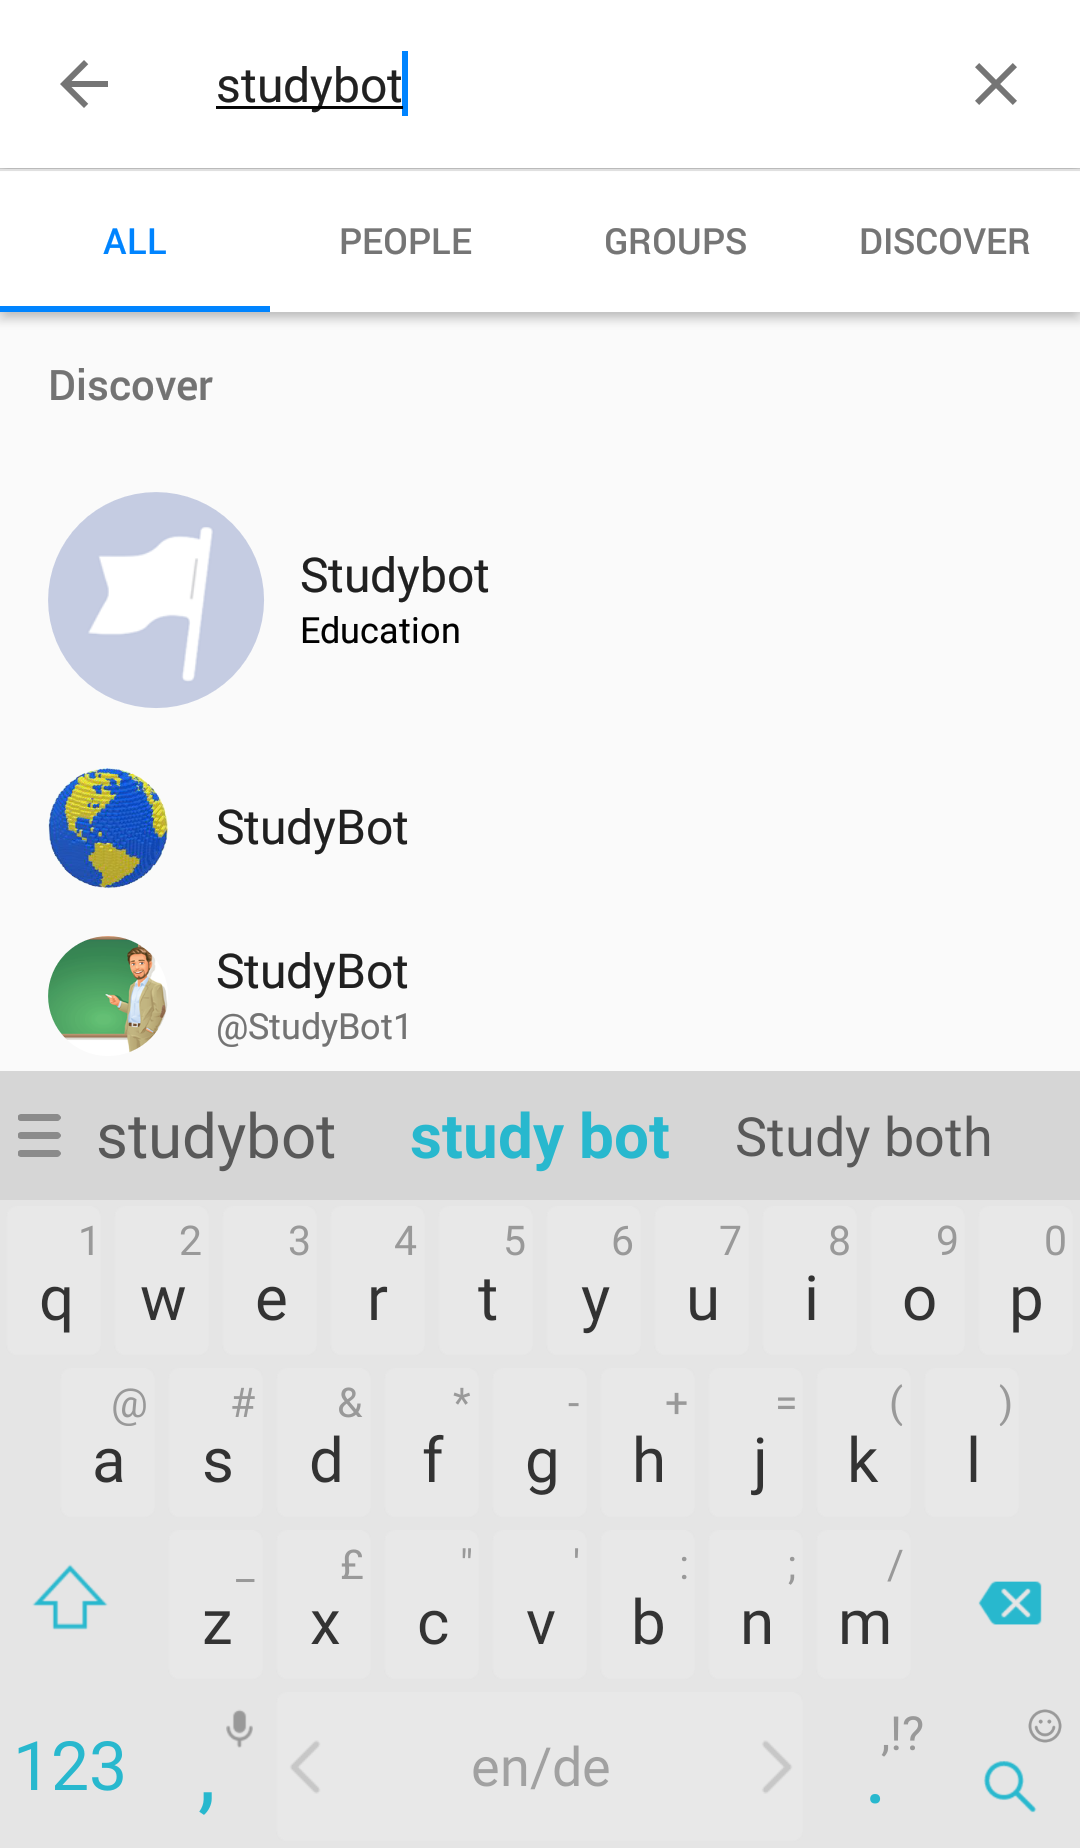
\includegraphics[width=0.28\textwidth]{images/interface/01-search.png}
	\caption{Search}
	\label{fig:01-search}
\end{wrapfigure}

At this point it is defined what the example chatbot is able to do,
and which technologies are used for its implementation.
\\

Before looking at the implemenation,
the usage of the chatbot is shown from a user's point of view.
\\
The following is a presentation of how this chatbot is used.
\\

Facebook Page and a Facebook Messenger bot have been created under the name \emph{Studybot}.
\\
By not publishing the Facebook Page, also the chatbot remains only accessible for administrators of the Facebook Page.
\\

The demonstration uses the Messenger Android application,
but Messenger bots can also be accesses through applications on other platforms
or using the web version of Facebook.
\\

When using the Messenger application as administror,
the bot can be found by using the search as shown in figure \ref{fig:01-search}.
\\

\begin{wrapfigure}{O}{0.3\textwidth}
  \centering
  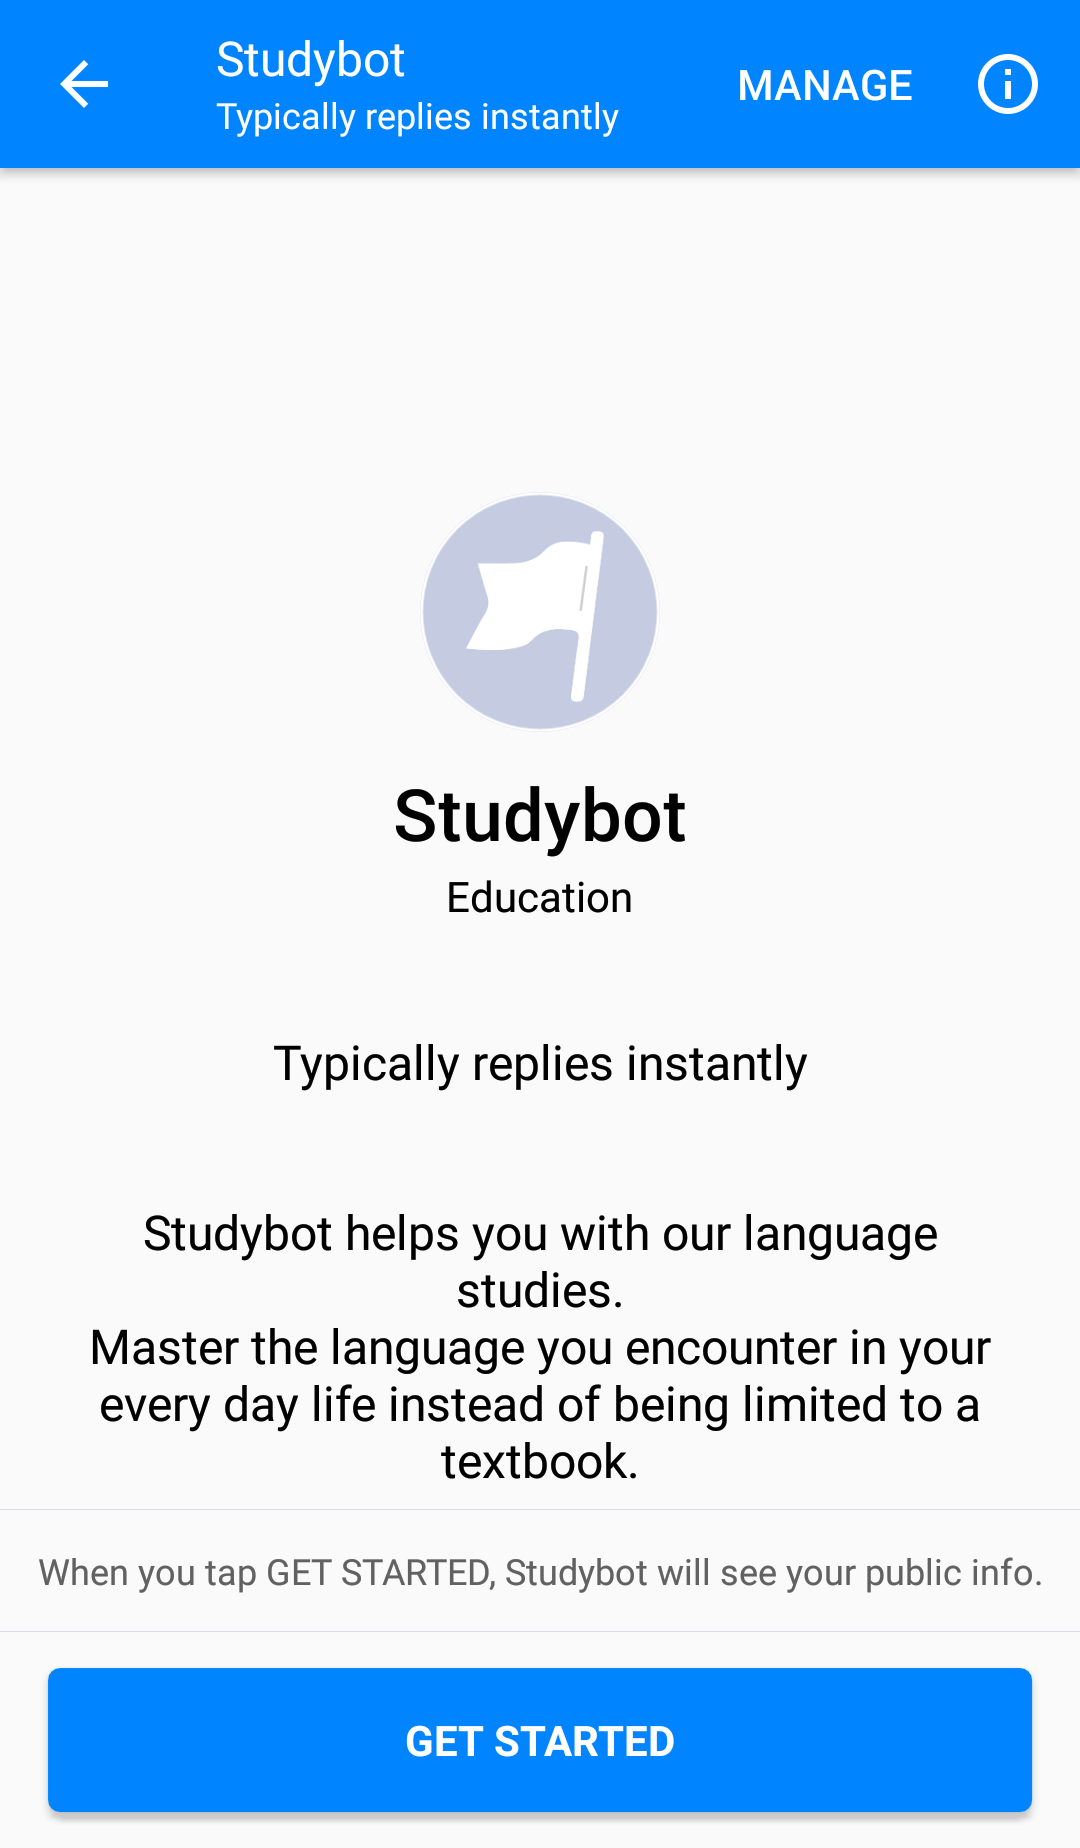
\includegraphics[width=0.28\textwidth]{images/interface/02-getstarted.png}
	\caption{Get Started Screen}
	\label{fig:02-getstarted}
\end{wrapfigure}

After navigating to the chatbot,
a description of the bot becomes visible.
This can be seen in figure \ref{fig:02-getstarted}.
\\
This view contains the profile image of the Facebook Page the chatbot belongs to,
the category the Facebook Page is part of,
and a text describing the functionality of the chatbot,
whereby all of these elements can be defined by the developer of the chatbot.
\\
A button labeled \textbf{Get Started} is displayed at the bottom of the view.
\\

\begin{figure}[h]
  \centering
  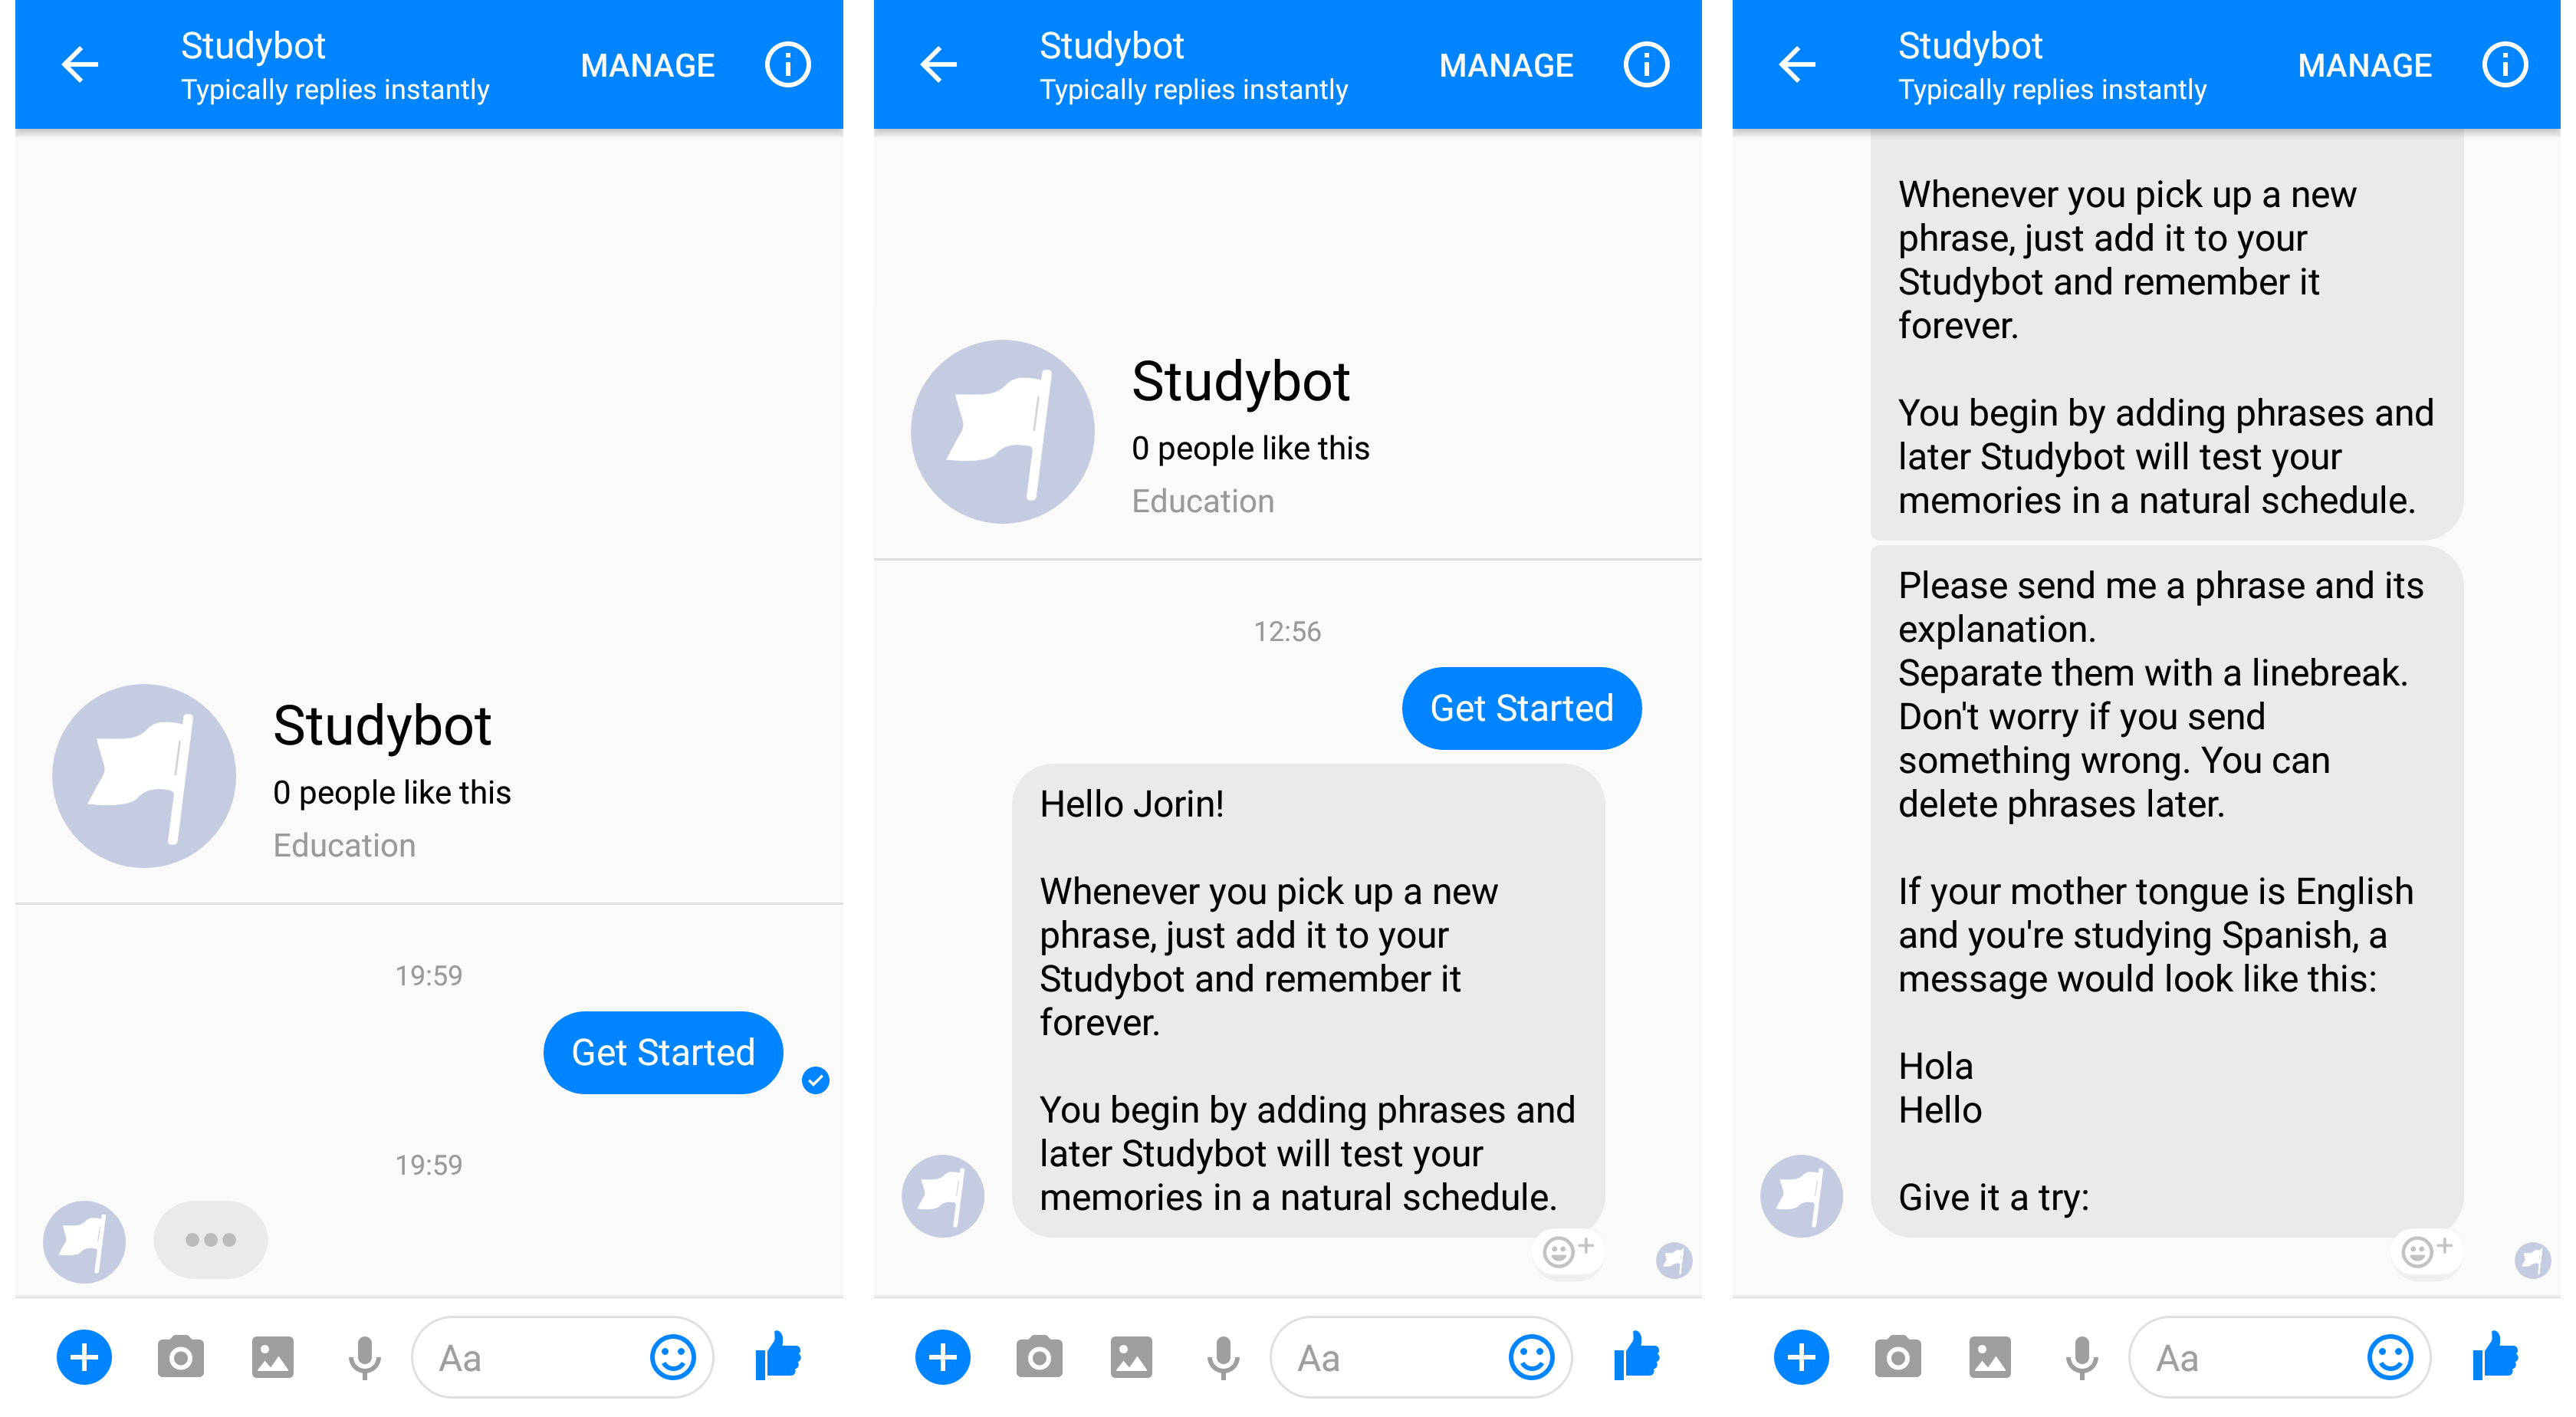
\includegraphics[width=0.9\textwidth]{images/interface/03-welcome.png}
	\caption{Messages introducing Studybot}
	\label{fig:03-welcome}
\end{figure}

When pressing the \textbf{Get Started} button, a message is sent to the chatbot,
and as indicated by the \emph{dots} visible in figure \ref{fig:03-welcome} in the left image,
the chatbot is active and about to send a reply.
\\
In normal conversations the \emph{dots} are used to indicated when a user is typing text.
\\
For chatbots the \emph{dots} indicated that the chatbot received the message and is crafting a reply.
\\

The image in the middle of figure \ref{fig:03-welcome} shows the first message sent to users;
users are greeted using their first name to create a more personal feeling atmosphere.
The greeting is followed by a two sentence long explanation of what this chatbot is doing.
\\
When working with text as a medium it is especially critical to focus only on the most important information;
with graphical elements and images users can perceive an impression with a single glace,
but to perceive the meaning of text the user needs to read word by word.
\\
Since in most scenarios the time users are willing to invest in understanding a product is limited,
every word in a text has to be selected carefully.
\\

It can be seen in the image on the right of figure \ref{fig:03-welcome} that a second message is sent to the user.
\\
The second message is delivered 5 seconds later that the first one to not overwhelm the users with too much information at once
by putting a \emph{wall of text} on their screen.
\\
This message contains instruction for the first step of using the application.
\\
The instructions are additionally illustrated by providing an example for a message in the expected format.
\\

\begin{figure}[h]
  \centering
  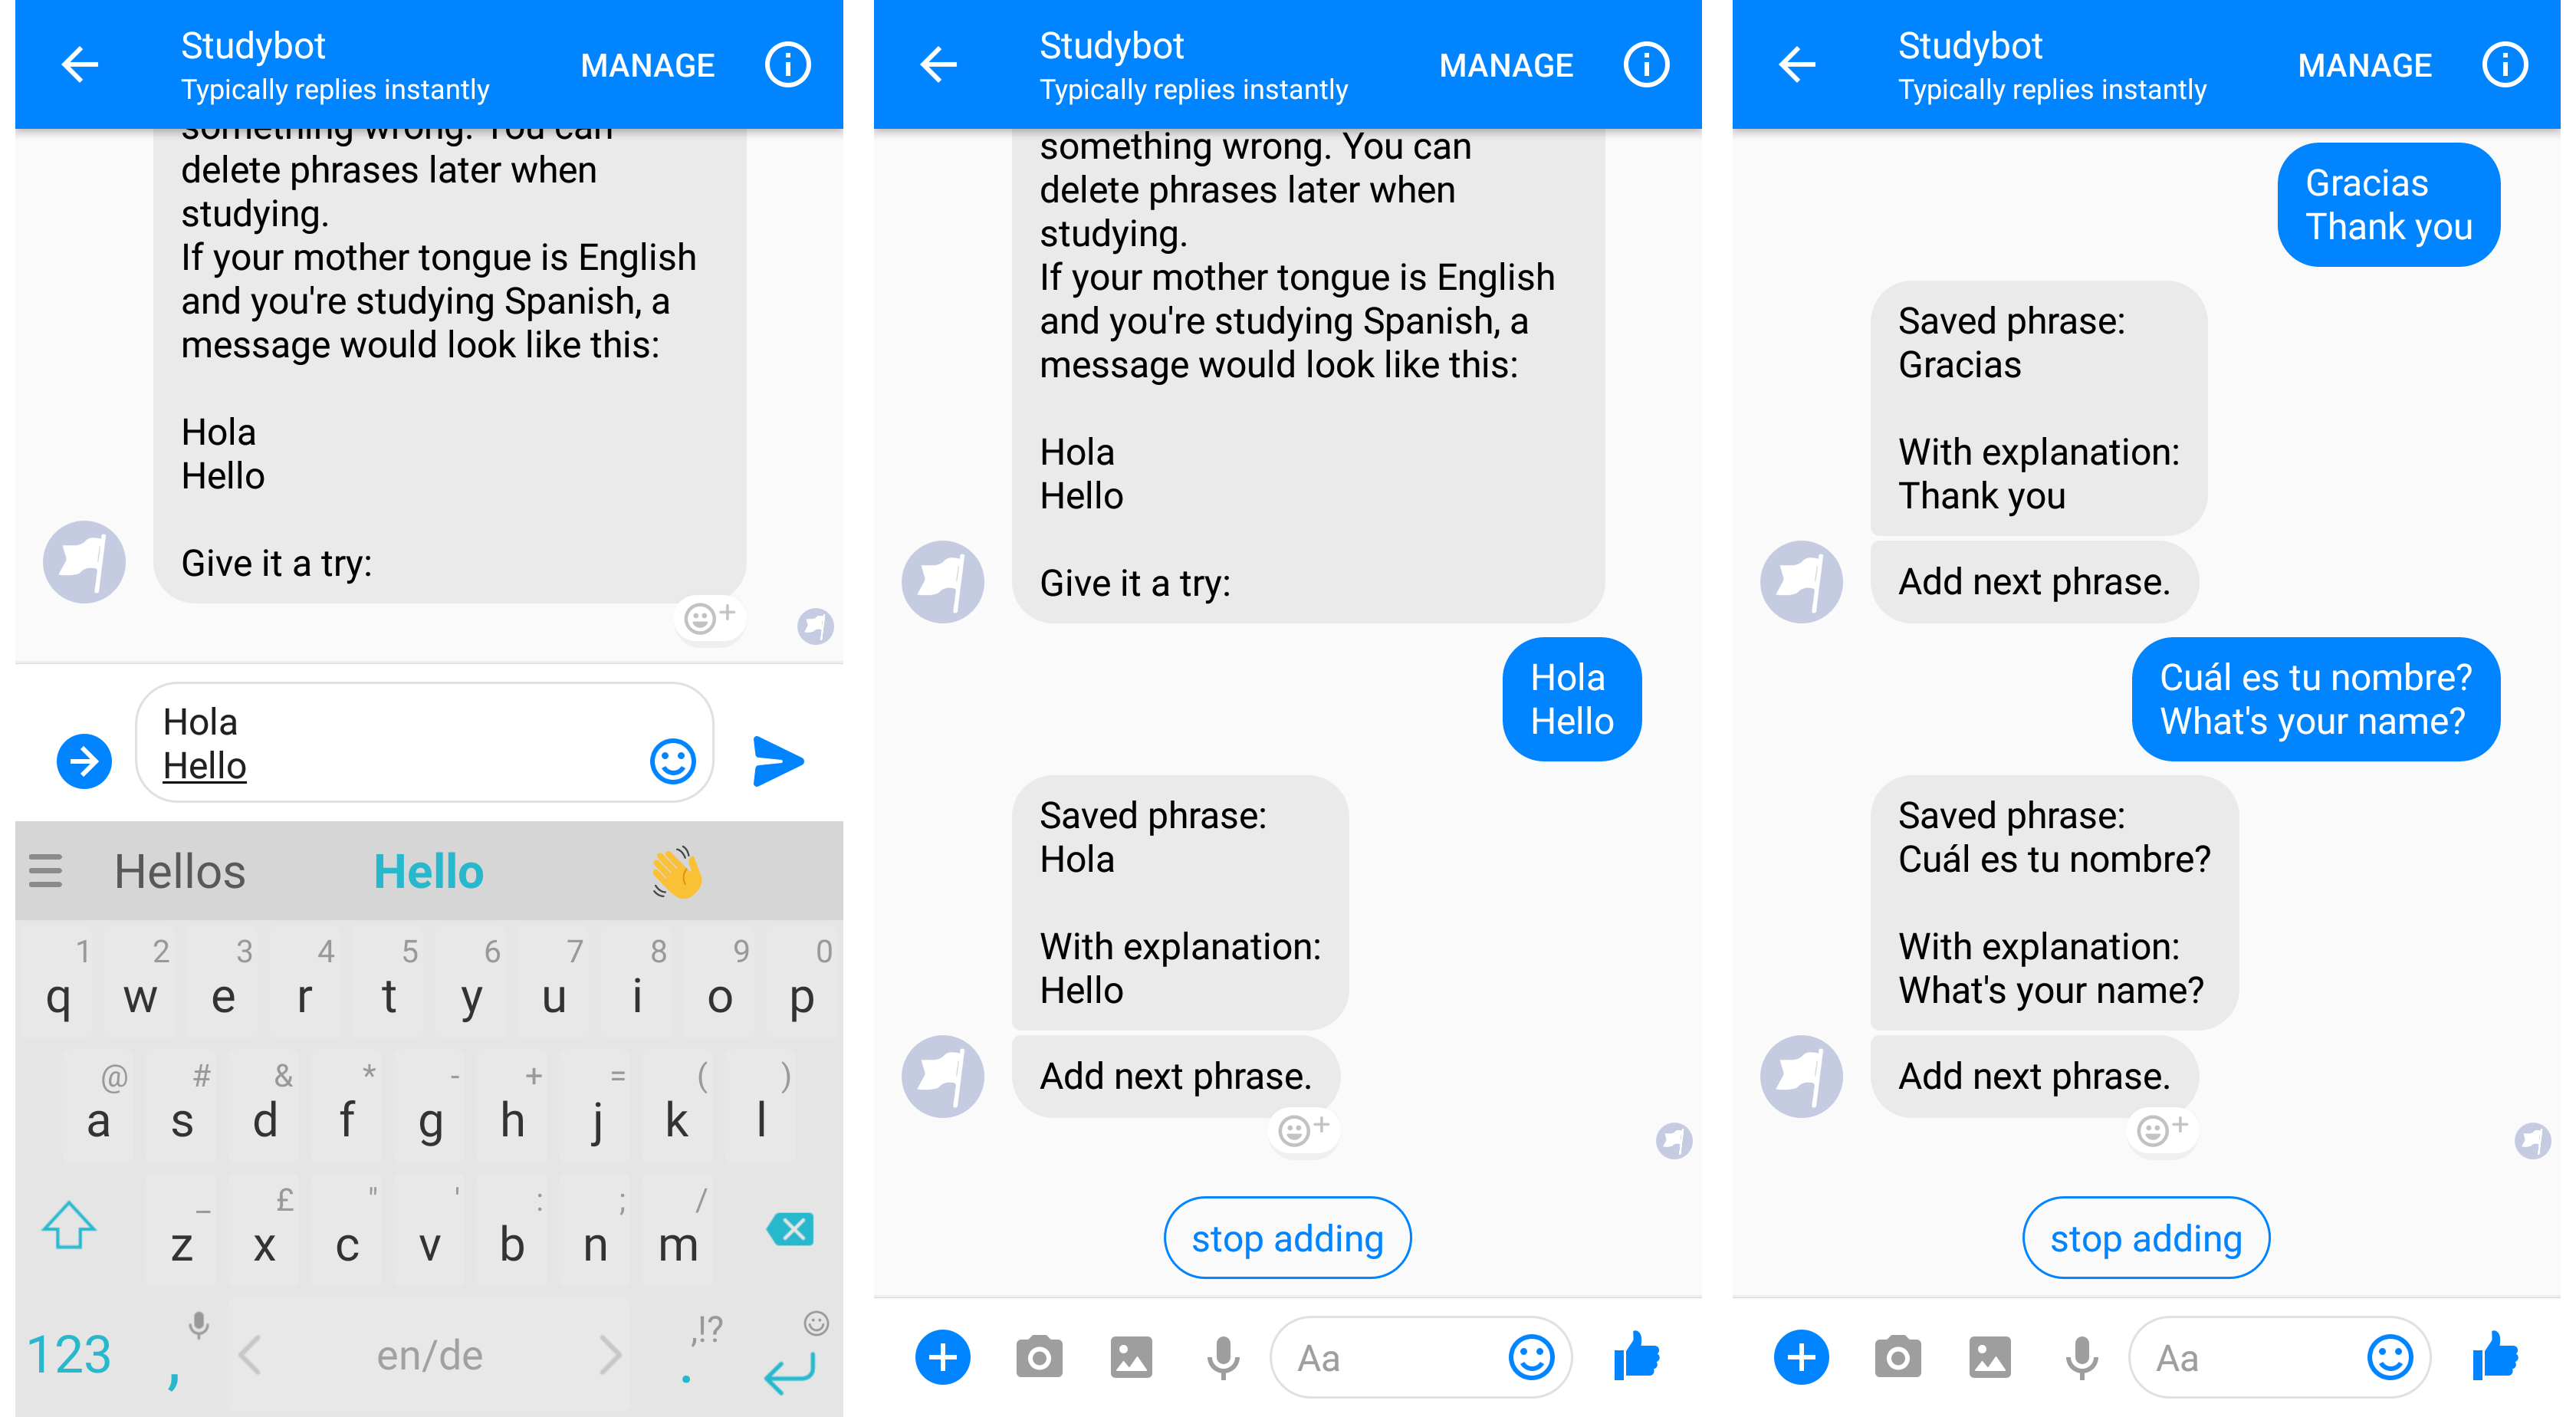
\includegraphics[width=0.9\textwidth]{images/interface/04-add.png}
	\caption{Adding three phrases}
	\label{fig:04-add}
\end{figure}

At this point the user needs to interact with the chatbot.
\\
Figure \ref{fig:04-add} shows how a user adds phrases to Studybot;
when typing a phrase, users first types the phrase in a foreign language they like to study,
then the \emph{return} or \emph{enter} key on the keyboard has to be used to insert a \emph{line-break},
and the next line contains an explanation for the preceding phrase.
\\
After the phrase is sent to the chatbot,
a confirmation message is displayed to keep the user updated about the current state of the system.
\\
This is followed by another message prompting the user to add more words.
\\
For a chatbot it is critical to always keep the user informed about the next expected action,
therefore a message should most of the time end with a prompt for a certain input or action.
\\

The image in the middle of figure \ref{fig:04-add} shows that this is the first point of the conversation,
that in addition to being able to type a reply, a button is displayed at the bottom of the messages,
which the user can use as an alternative way for interacting with the chatbot.
\\

\begin{wrapfigure}{O}{0.3\textwidth}
  \centering
  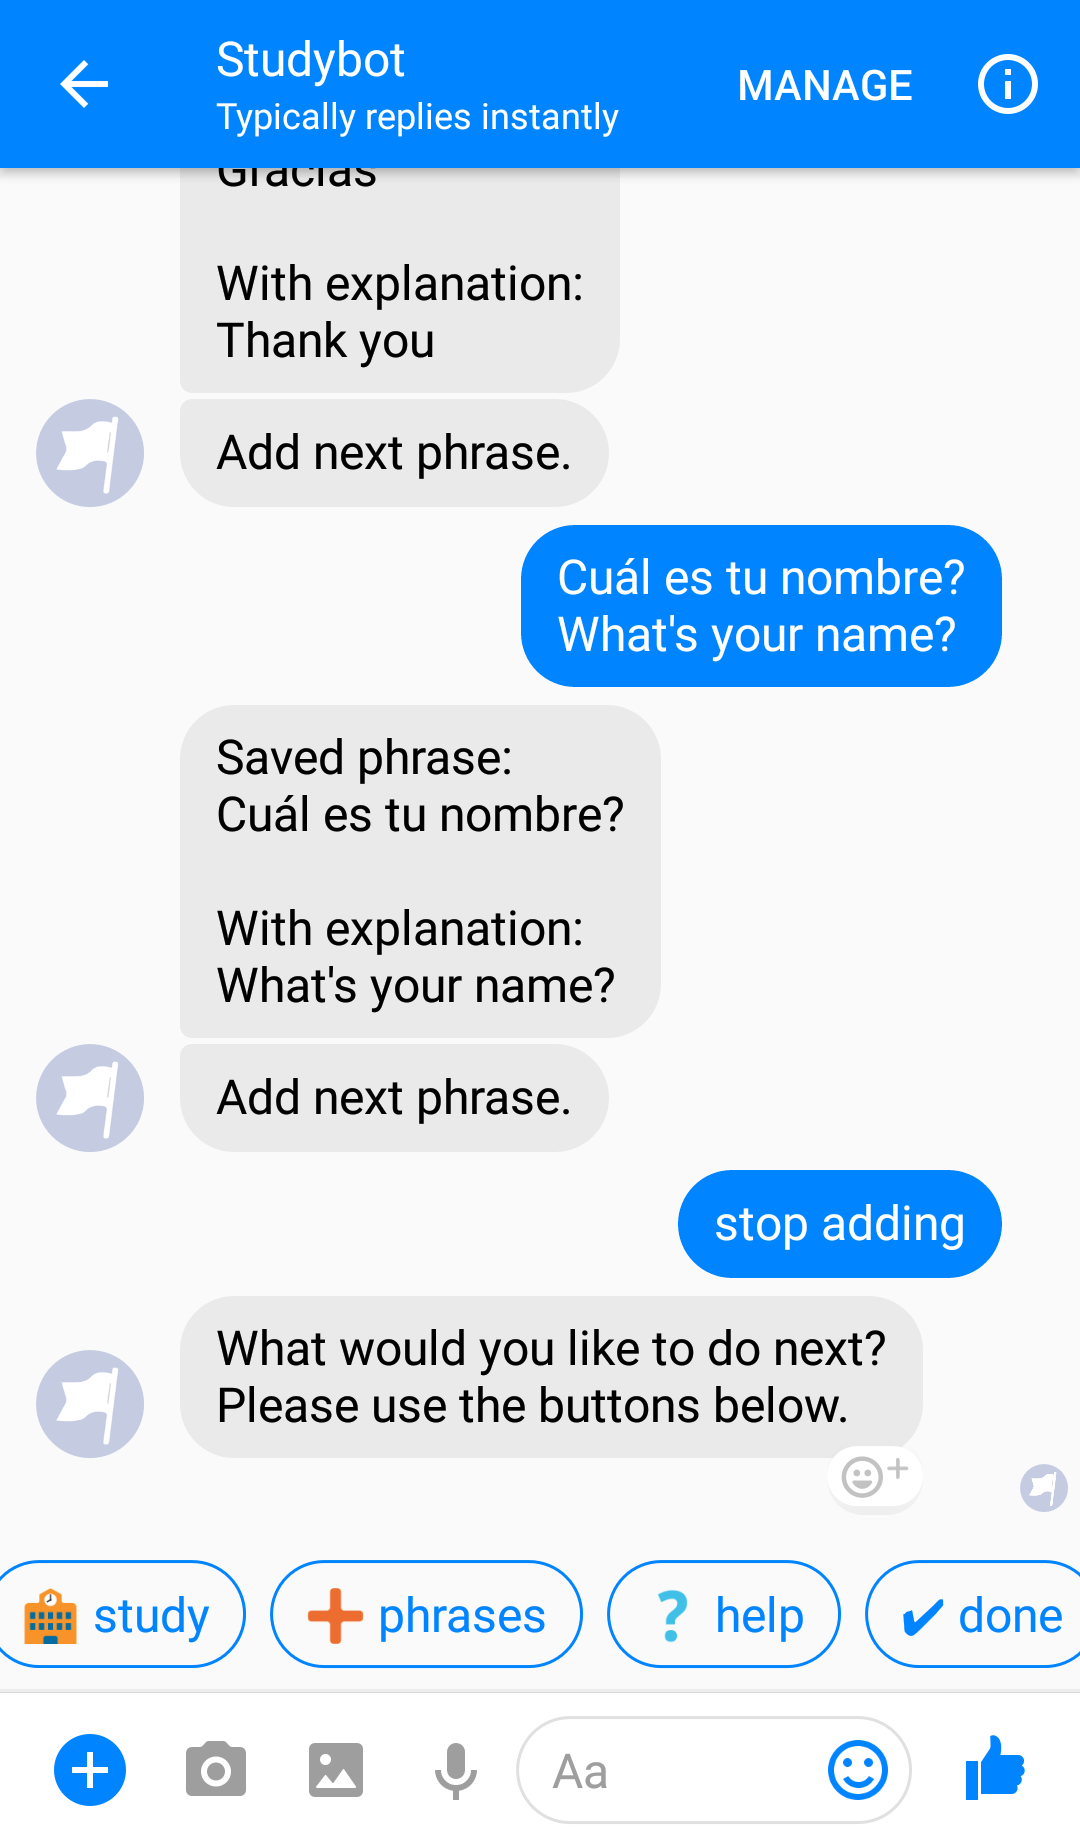
\includegraphics[width=0.28\textwidth]{images/interface/05-stop-adding.png}
	\caption{Stop adding phrases}
	\label{fig:05-stop-adding}
\end{wrapfigure}

As shown in figure \ref{fig:04-add}, three phrases have been added to Studybot
before the user decides to press the button labeled as \textbf{stop adding}.
\\
Figure \ref{fig:05-stop-adding} shows, that after stopping the adding of phrases the user is prompted with an array of four possible actions;
the actions are labeled as \textbf{study}, \textbf{+ phrases}, \textbf{help} and \textbf{done} respectively
and each button label also contains an emoji\footnote{``Emoji are pictographs (pictorial symbols) that are typically presented in a colorful form and used inline in text. They represent things such as faces, weather, vehicles and buildings, food and drink, animals and plants, or icons that represent emotions, feelings, or activities.''\cite{emoji}} used as icon for the action to make it easier identifiable for the user.
\\

The chatbot has different modes of interaction.
\\
Internally the chatbot needs to keep track of the current mode of each user to be able
to address messages in the correct context.
\\
In figure \ref{fig:05-stop-adding} the user has left the mode for adding words
and entered the \emph{menu mode} from where other modes can be accessed.
\\

\begin{figure}[h]
  \centering
  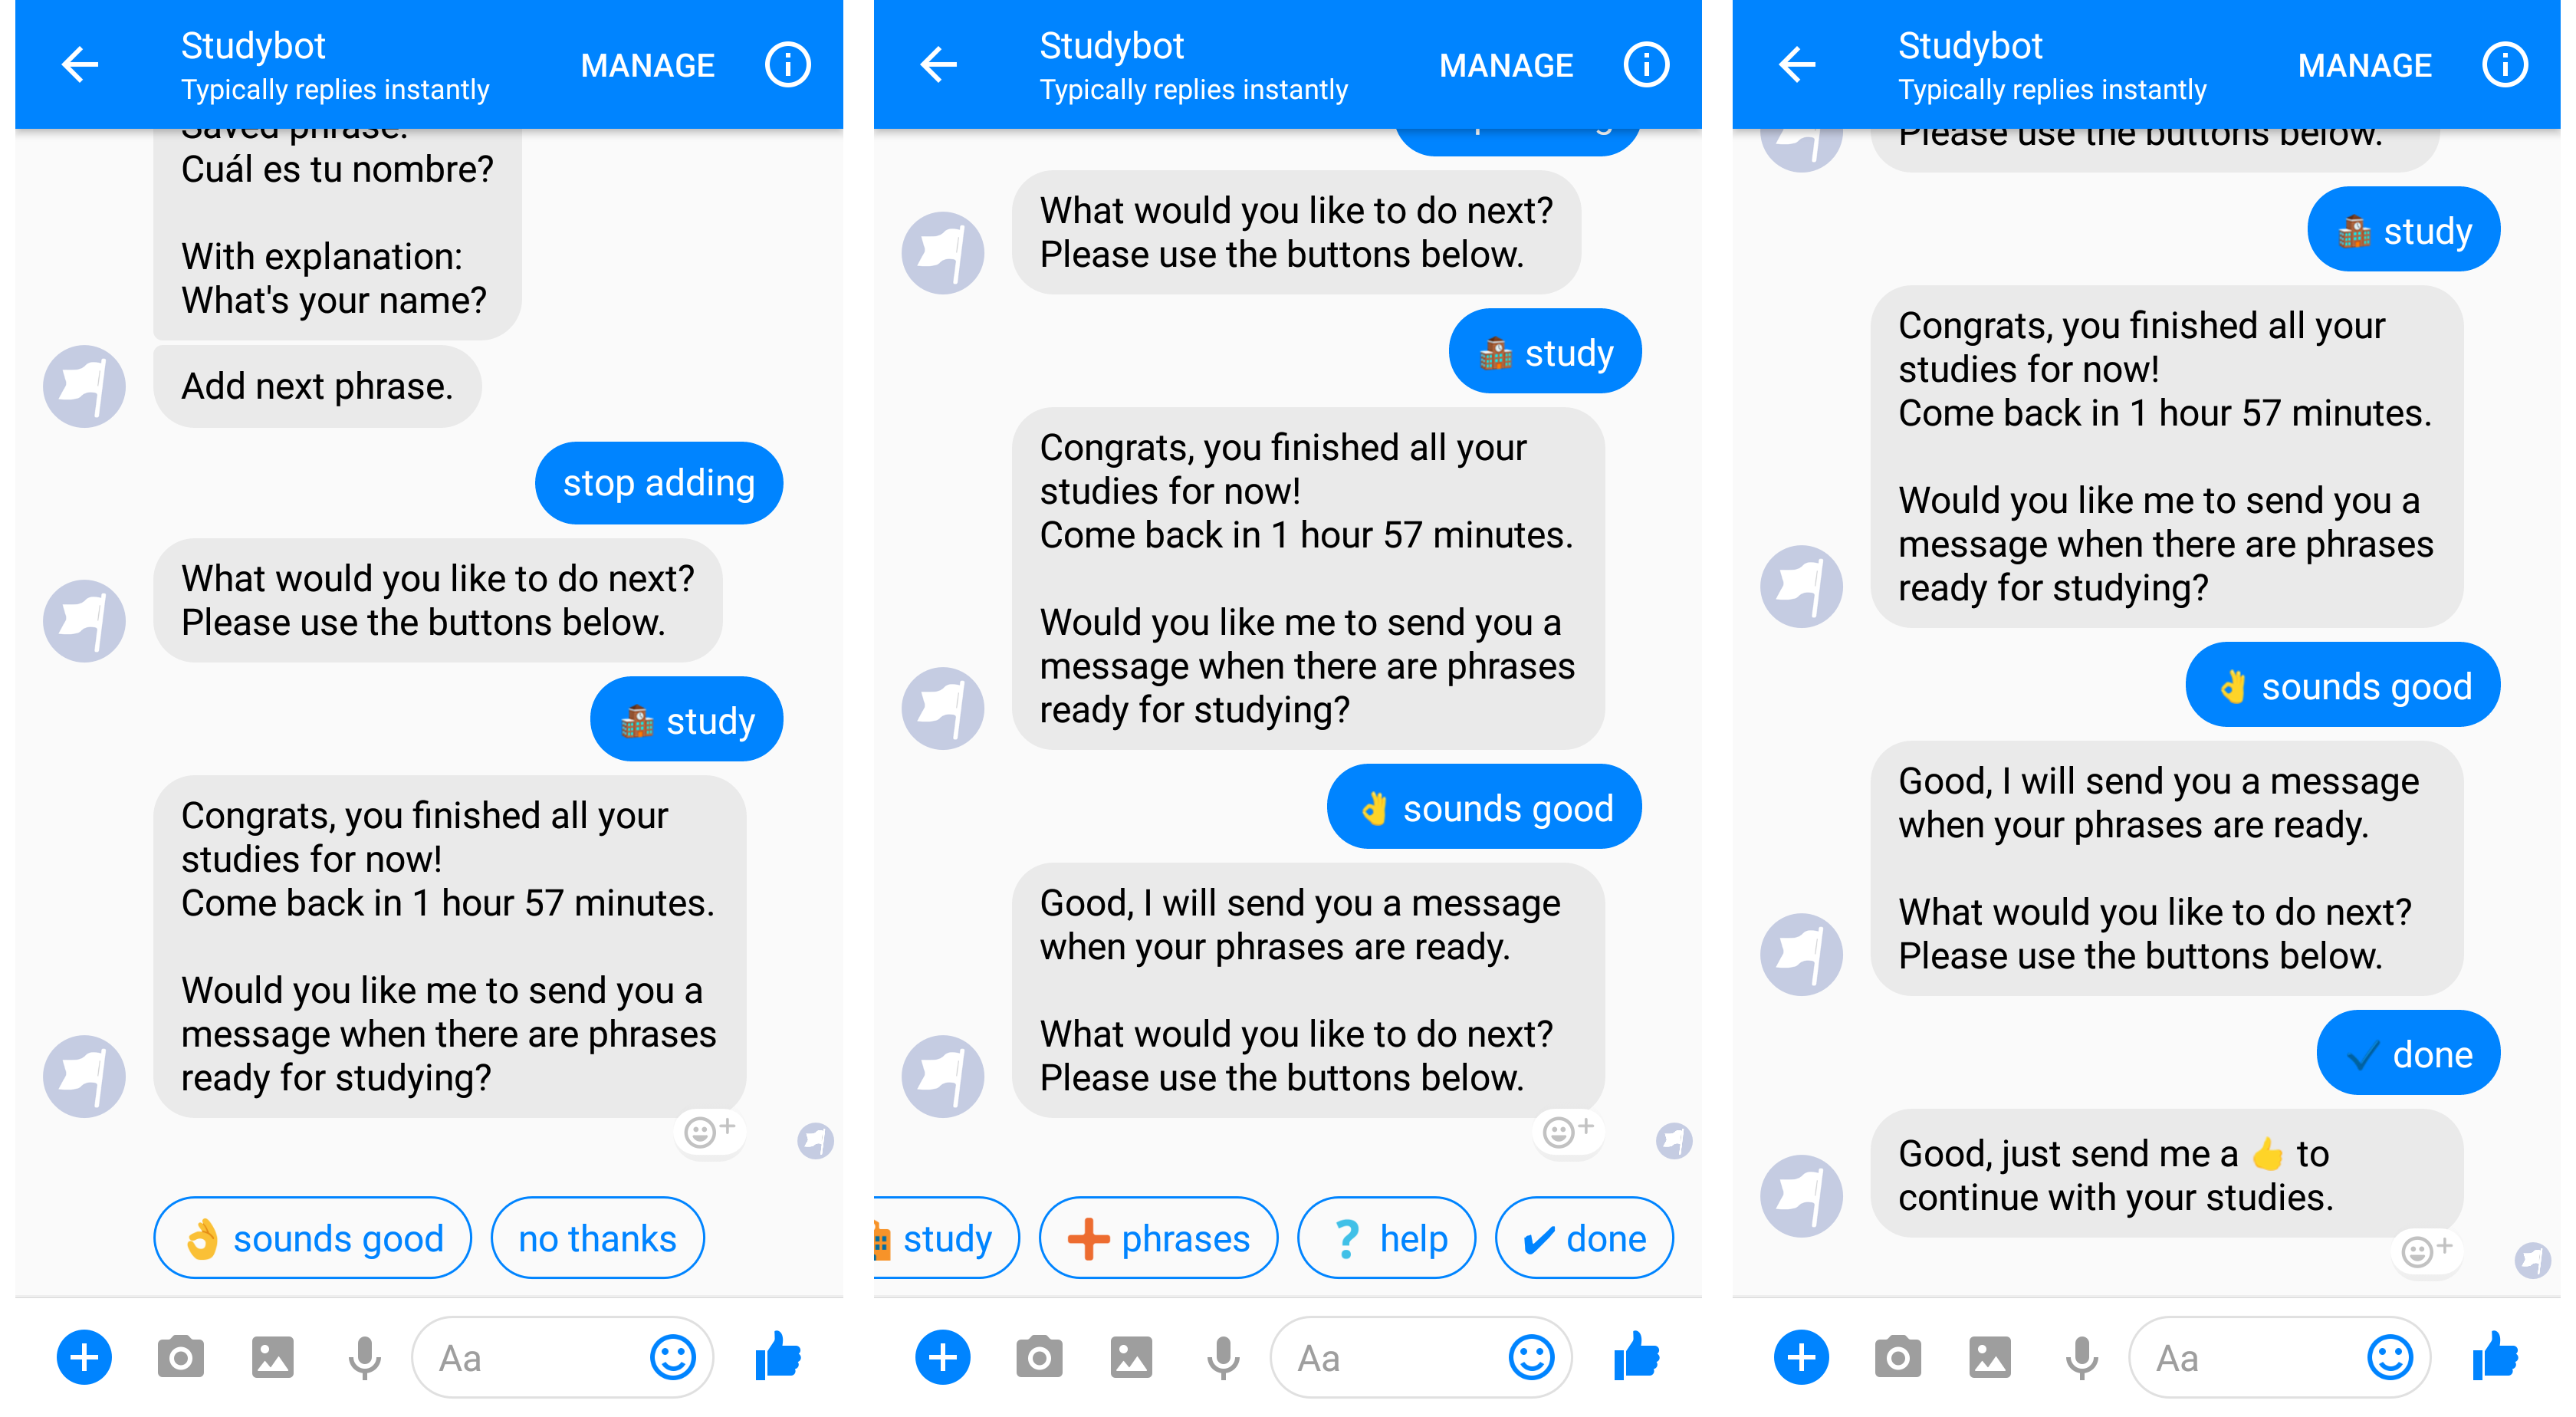
\includegraphics[width=0.9\textwidth]{images/interface/06-enable-notify.png}
	\caption{Attempt to study and activation of notifications}
	\label{fig:06-enable-notify}
\end{figure}

By clicking on the button labeled \textbf{study},
the user switches to the mode for studying of the added vocabulary.
\\
However as the image on the left of figure \ref{fig:06-enable-notify} shows,
the added phrases cannot be studied yet.
\\

Studybot uses a concept known as \emph{spaced repetition system}, or short \emph{SRS},
which is described as ``a learning technique that incorporates increasing intervals of time between subsequent review of previously learned material in order to exploit the psychological spacing effect.''\cite{srs}
\\
Based on this approach users need to wait before studying newly added vocabulary.
The more often a phrase is guessed correctly the less frequent the user will be asked to review the phrase.
\\

\begin{figure}[h]
  \centering
  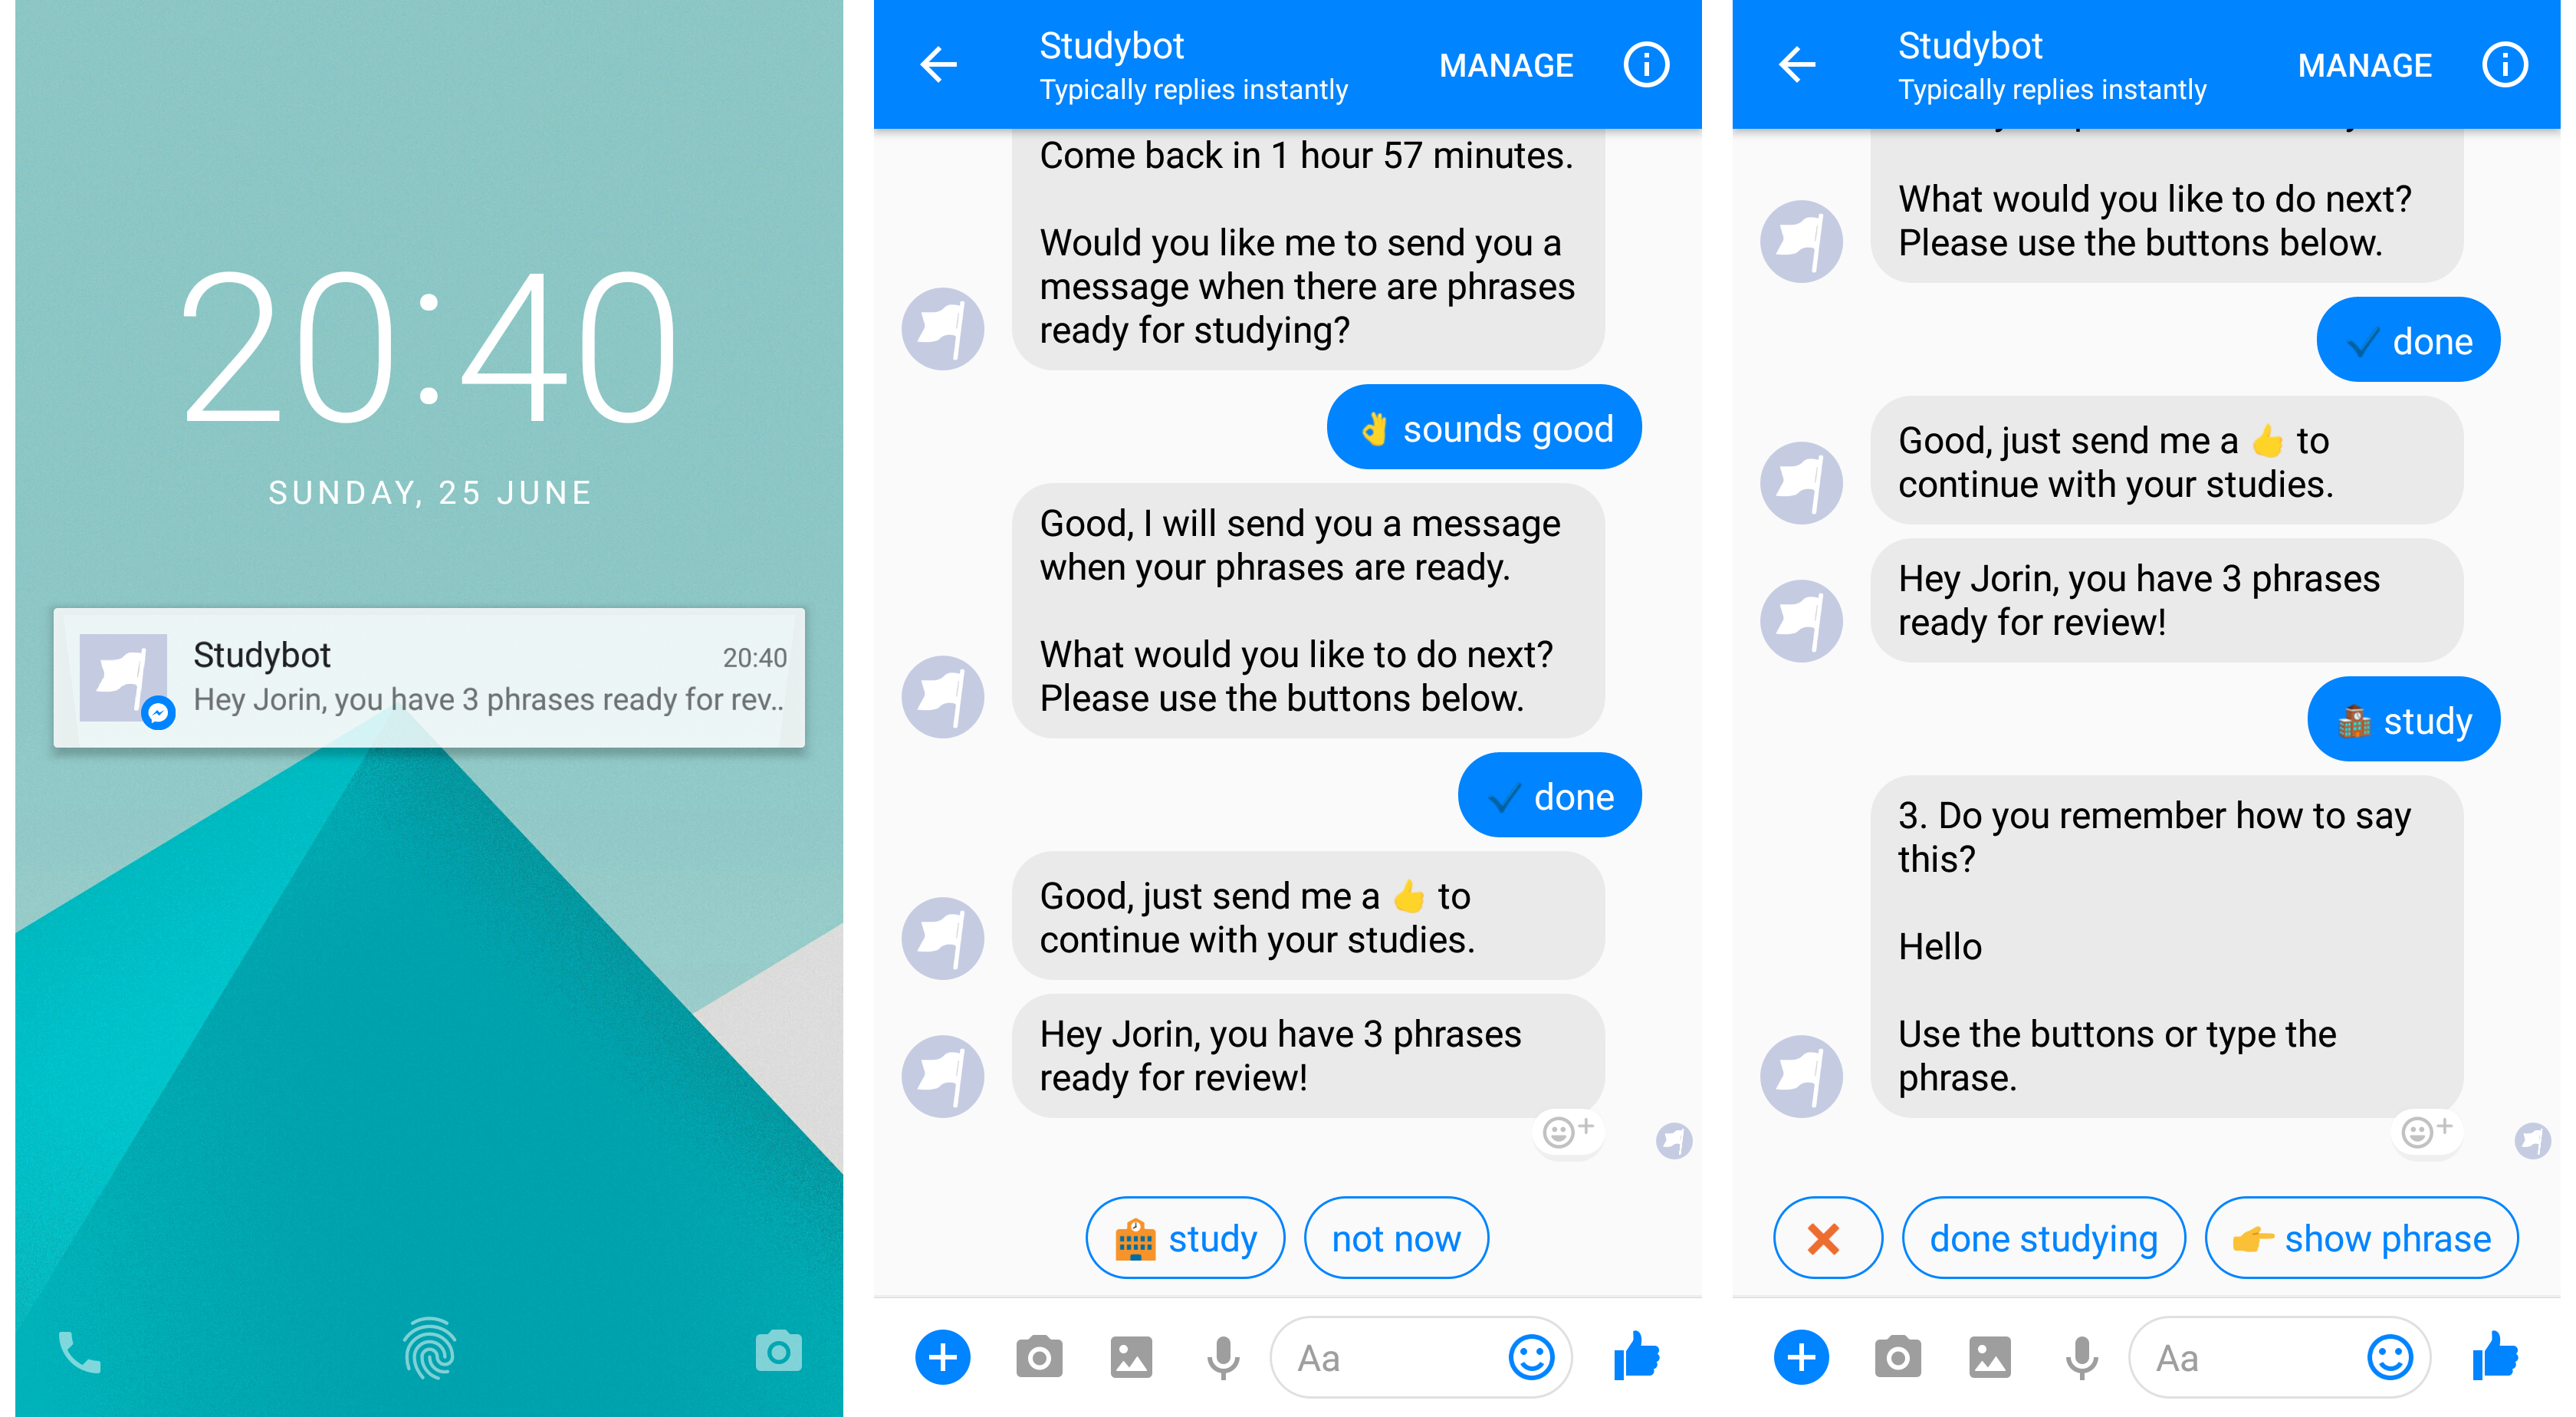
\includegraphics[width=0.9\textwidth]{images/interface/07-notify-study.png}
	\caption{Notification message and beginning of study}
	\label{fig:07-notify-study}
\end{figure}

Instead of studying the previously added phrases directly,
the user is offered to receive a notification message once phrases are ready for review.
\\

When sending notifications to users, it is important to not send more messages than necessary,
and depending on the messenger platform, there are different policies in place on how many messages are permitted.
\\
The platform policy of Facebook Messenger clearly states to
``respect all requests (either on Messenger or off) by people to block, discontinue, or otherwise opt-out of your using Messenger to communicate with them''\cite{fbpolicy},
which means there needs to be a way for users to disable the sending of notifications;
and further the platform policy clarifies that ``you may message people within 24 hours of a person's interaction with your business or Bot ..., and until the next interaction, you may send one additional message after this 24 hour period in order to follow up on your conversation.''\cite{fbpolicy}
\\

\begin{figure}[h]
  \centering
  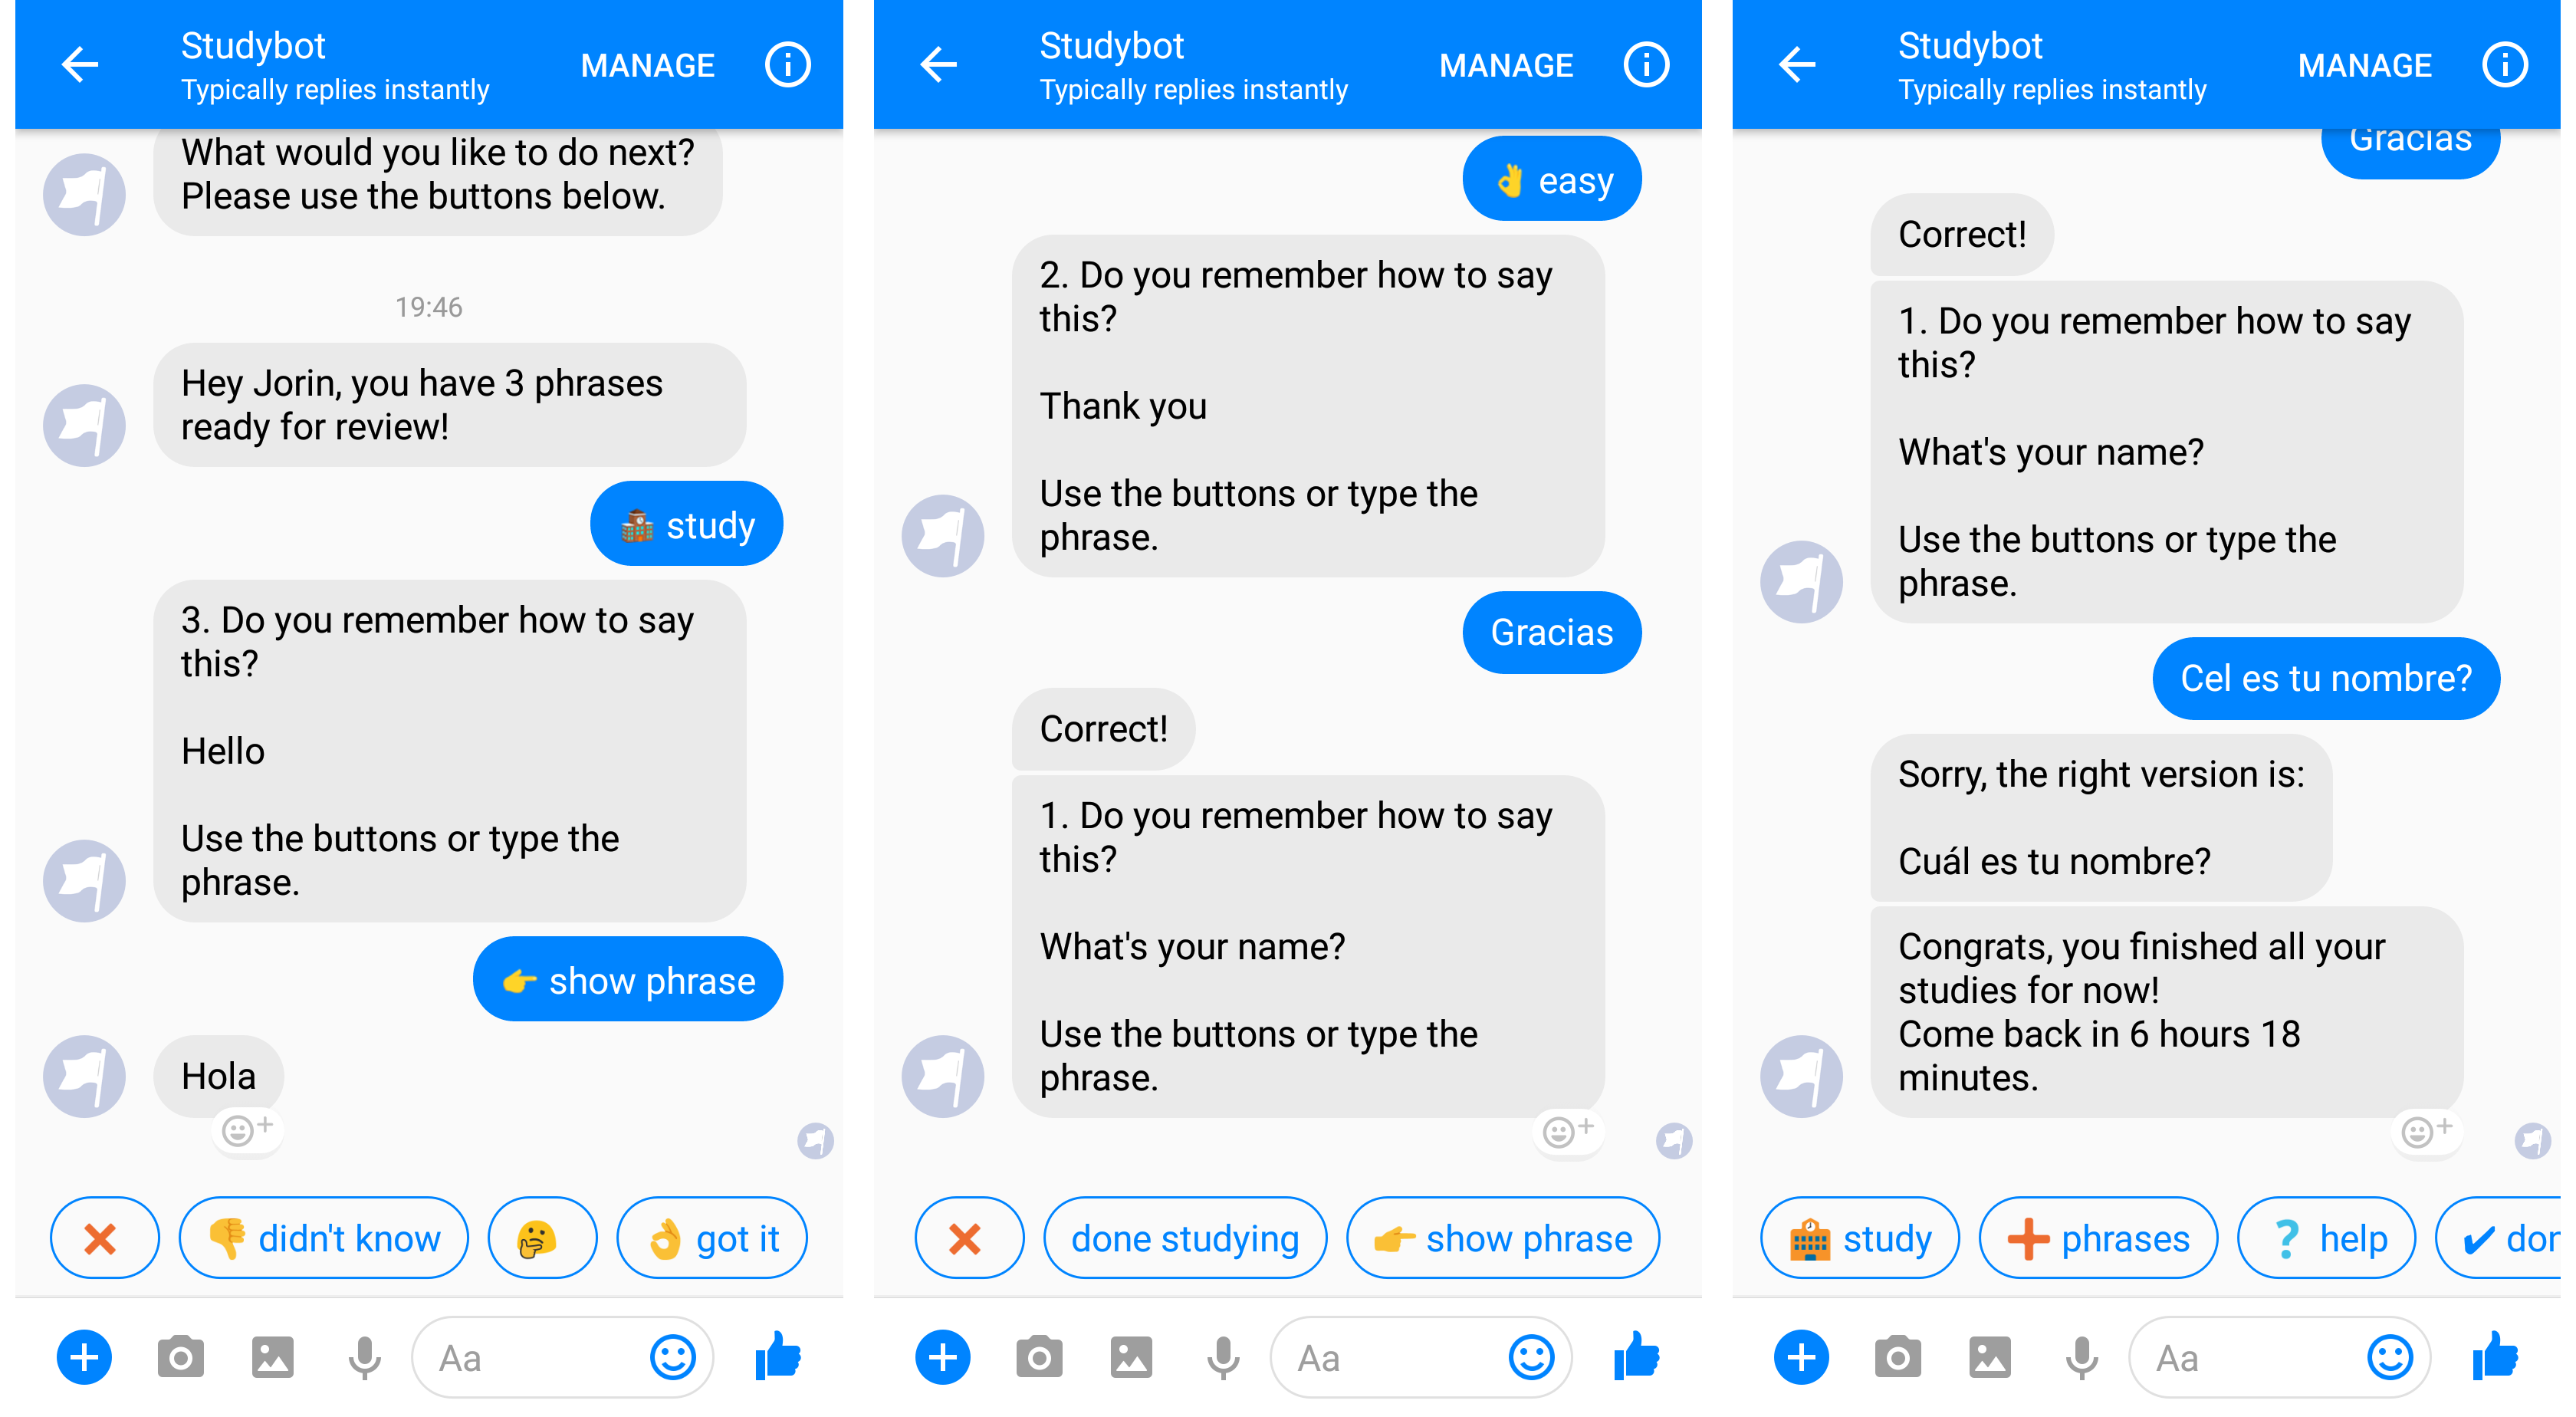
\includegraphics[width=0.9\textwidth]{images/interface/08-study-done.png}
	\caption{Study using buttons or by typing}
	\label{fig:08-study-done}
\end{figure}

In figure \ref{fig:07-notify-study} a notification on form the Messenger application on the mobile phone is how.
It is triggered when studies are ready for review.
\\
When opening the conversation with the chatbot,
the user is now prompted to study.
\\
As defined as a requirement in \ref{funcreq} on page \pageref{funcreq},
while studying one is free to choose to answer either by using the buttons at the bottom of the screen
or by directly typing the correct phrase.
\\

The \textbf{x} button available on the right image of figure \ref{fig:07-notify-study},
allows users to delete a phrase.
\\
Since there is no possibility in Facebook Messenger to display a long list of interactive elements to the user,
creating separate functionality for editing and deleting phrases is difficult to achieve,
and while studying is at this point the only possibility to refer to a phrase.
\\

The figures \ref{fig:07-notify-study} and \ref{fig:08-study-done} show a subtle decision to display the buttons users are most likely to interact with,
on the right side;
in other places it is more intuitive to show the most important information on the left,
since English language is written from left to right and we scan text accordingly;
however for certain interactions, like studying in this case, need to be performed so frequently,
a user will remember the location of the buttons quickly and doesn't need to scan process the information every single time.
\\
In this case it is helpful to have the most used action on the right side, since the majority of humans is right-handed,
therefore can reach the button with the thumb with less effort when using a mobile phone single-handed.
\\


With this the primary interactions for the example chatbot are covered.
\\
Many of the implemented interactions can be transfered and reused when creating other kinds of chatbot;
addressing the user by name,
sending text in small chunks with a time of delay in between,
prompting the user for specific input with every message,
keeping track of the user's context,
asking for permission before sending notifications and
consciously ordering buttons,
these patterns can be applied in many different scenarios.

% TODO
% Information about secondary interactions can be found on \pageref{fig:secondary} in the appendix.

